\scanpage{100}
\diagram{\begin{tikzcd}[ampersand replacement=\&,row sep=small]
 D^{\deleted{\unsure{i|1}}}\mathbin{.}C\geq0\qquad\text{si}\qquad C>0\arrow[d,Rightarrow,"?"]\\
 D^iX_i\geq0\qquad\text{si}\qquad X_i>0\qquad ??
\end{tikzcd}}
\[
 D^{\deleted{\unsure{1|i}}}\in P_1^{+\circ}\Longrightarrow D^i\in P_i^{+\circ}
 \qquad\text{pour}\quad i\leq d-1\qquad\uline{\text{hyp. de réc.}}
\]
\[
 \deleted{\unsure{D^2|D^d}}\qquad\text{\unsure{aura-t-on}}\qquad
 D^d\in P_d^{+\circ}\quad\text{i.e.}\quad D^d\geq0\quad ??
\]
\[
 \text{On a}\qquad D^d =
 \underset{\substack{\rotatebox{-90}{$\in$}\\P_i^{+\circ}}}{D^i}
 \underset{\substack{\rotatebox{-90}{$\in$}\\P_{d-i}^{+\circ}}}{D^{d-i}}
 \qquad (0<i<d)
\]

\diagram{\begin{tikzcd}[ampersand replacement=\&,row sep=small,column sep=small]
 \boxed{P_i^{+\circ}\mathbin{.}P_{d-i}^{+\circ}\geq0\quad ?}\arrow[d,Leftrightarrow] \&
 P_i^{+\circ}P_j^{+\circ}\subset P_{\unsure{i\mathrm e j|i+j}}^{+\circ}\arrow[l,Rightarrow]\\
 \boxed{\alpha_i(P_i^{+\circ})\subset P_{d-i}^+}\arrow[d,Leftrightarrow]\&\\
 \boxed{\alpha_{d-i}(P_{d-i}^{+\circ})\subset P_i^+}\&
\end{tikzcd}}

\diagram{\begin{tikzcd}[ampersand replacement=\&,row sep=small]
 D\mathbin{.} C\geq0\qquad\text{si }C\geq0\\
 D^2\mathbin{.}\deleted{\unsure{D_i|D}}\mathbin{.}D'\geq0\qquad\text{si }D'\geq0\arrow[d,Rightarrow,"?"]\\
 D^3\geq0
\end{tikzcd}}
\figure{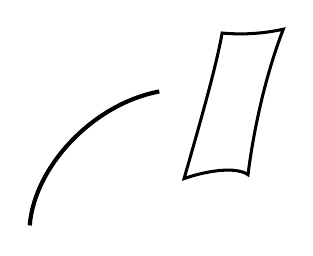
\begin{tikzpicture}[x=.70cm,y=.70cm]
 \draw[line width=1.5pt] (0,0) .. controls (.08,1.05) and (1.13,2.20) .. (2.35,2.43);
 \draw[line width=1.1pt] (2.80,.85) .. controls (3.05,1.72) and (3.38,2.86) .. (3.49,3.49)
 .. controls (3.83,3.46) and (4.19,3.47) .. (4.60,3.56)
 .. controls (4.24,2.63) and (4.04,1.58) .. (3.96,.92)
 .. controls (3.75,1.07) and (3.23,1.00) .. cycle;
\end{tikzpicture}}
\diagram{\begin{tikzcd}[ampersand replacement=\&]
 P_1^{+\circ}\subset\unsure{\mathcal A|A}^1\arrow[r]\&\mathcal A_2\supset P_2^+
\end{tikzcd}}
\[
 \deleted{\unsure{D+n|D+}}\qquad D'+nD\in P_2^+
\]
\[
 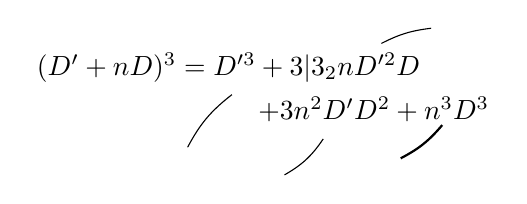
\begin{tikzpicture}[x=1em,y=1em]
 \node[anchor=base west] at (0,1.6) {$(D'+nD)^3=D^{\prime 3}+\unsure{3|3_2}nD^{\prime 2}D$};
 \node[anchor=base west] at (8.0,0) {$+3n^2D'D^2+n^3D^3$};
 \draw (12.8,2.75) to[bend left=10] (14.6,3.3);
 \draw[thin] (5.8,-1.0) to[bend left=12] (7.4,.9);
 \draw[thin] (9.3,-2.0) to[bend right=13] (10.7,-.7);
 \draw[thick] (13.5,-1.4) to[bend right=11] (15,-.2);
 \end{tikzpicture}
\]
\figure{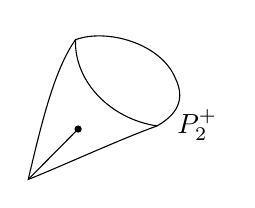
\begin{tikzpicture}[x=.66cm,y=.66cm]
 \draw (.05,0) .. controls (.31,1.10) and (.55,2.11) .. (.96,2.69)
 .. controls (1.57,2.91) and (2.60,2.62) .. (2.88,1.95)
 .. controls (3.14,1.43) and (2.75,1.16) .. (2.53,1.03)
 .. controls (1.83,.78) and (.68,.25) .. cycle;
 \draw (.96,2.69) .. controls (.93,1.88) and (1.64,1.16) .. (2.53,1.03);
 \draw (.05,0)--(1.01,.97); \fill (1.01,.97) circle (.07);
 \node[right] at (2.73,1.05) {$P_2^+$};
\end{tikzpicture}}
\[
 \begin{aligned}
 &\deleted{D+\tfrac1nD'}\\
 &D'+nD\simeq
 \end{aligned}
 \qquad\boxed{D^3\geq0}
\]
% archive sheet number: 99
